\chapter{Softwareentwicklungsumgebung}
\label{ch:chapter04}

\section{Veränderung der Rahmenbedingungen}

Die Entwicklung eines flexiblen und skalierbaren Systems und Umgebung für die Softwareentwicklung innerhalb von Banken erfordert wesentliche Veränderungen in den Strukturen der IT-Bereiche der Institute und in ihrem Ablauf. Wesentlicher Faktor ist hierfür die Tatsache, dass die Anwendungen und Systeme für die Softwareentwicklung ständigen Veränderungen ausgesetzt sind. Standards in der Softwareentwicklung sind mittlerweile agil und verändern sich kontinuierlich und dynamisch. Eine flexible IT-Architektur ist erforderlich, um sich diesen Veränderungen anzupassen.
\medskip
\\
Bussmann et al. nennt zwei Wege für den Ersatz und grundlegenden Re-Design von Kernsystemen: \cite{Bussmann2006}
\begin{itemize}
    \item Anwendungen schrittweise entkernen, erneuern und modularisieren und funktionale Anforderungen konsolidieren
    \item Kernsysteme durch völlig neue, selbst entwickelte Applikationen austauschen oder einsetzen von Standardsoftware
\end{itemize}
%

\paragraph{IT als Kernkompetenz} Bussmann et al. bezeichnet die IT als Kernkompetenz. IT-Anwendungen unterscheiden sich in zwei Bereiche, in welcher Technologietrends zu innovativen Lösungen führen. Neben den Anwendungen für den Dialog mit Kunden sind es Anwendungen zur Steuerung und Unterstützung von internen Prozessen, die gerade im Finanzwesen mit steigenden Anforderungen nicht mithalten können. \cite{Bussmann2006}
\medskip
\\

\paragraph{Relevanz der BaFin Anforderungen für Entwickler}
Die BaFin Anforderungen, Gängige Sicherheitsstandards und weitere Vorschriften sind für Entwickler wichtig, um ihre Verantwortung über die IT-Risiken in Banken und anderen systemrelevanten Betrieben zu verstehen. Insbesondere sind sie für die Entwicklung nachvollziehbarer Systeme für ihren nachhaltigen Betrieb, Überwachung und Überprüfung zu berücksichtigen. Um verwachsene und unflexible Architekturen zu vermeiden sollten Entwickler, im Bereich der Anwendungen, die interne Prozesse unterstützen \cite{Bussmann2006}, sich mit diesem Thema auseinandersetzen.

Neben den Leistungsansprüchen sollten die Sicherheitsansprüche im Vordergrund stehen. Die Implementierung von neuen Technologien wirft bei wesentlichen Veränderungen viele Compliancefragen auf \cite{MaRisk:2017}. Diese hängen mit den Sicherheitsansprüchen zusammen. 

\paragraph{Idee für ein innovatives Risikomanagement}
Die von Disterer beschriebenen Probleme im Betrieb von Anwendungen durch die mangelnde Beachtung von nichtfunktionalen Anforderungen und die Einführung von Quality Gates \cite{mci/Disterer2011} kann hierbei auf Probleme für die internen Kontrollverfahren ausgeweitet werden. Eine Koordination zwischen Entwicklung und Betrieb sollte das IT-Risikomanagement miteinbeziehen. Dabei darf die Geschwindigkeit des Entwicklungs- oder Integrationsprozesses nicht beeinträchtigt werden. Die Schnelligkeit hat bei der Beantwortung von Compliancefragen eine wichtige Rolle. Entwickler könnten zuerst die Prozesse des IT-Risikomanagements optimieren und automatisieren, um sich Handlungsfreiheit für Innovation und wesentlichen Veränderungen innerhalb der Organisation zu schaffen. Sie sollten in das Risikomanagement integriert werden. Ein Entwickler aus einem anderen Projekt könnte als Compliance- und Risikoverantwortlicher parallel wichtige Compliancefragen auf technischer Ebene schnell überprüfen und vorab beantworten. Dadurch könnte unter Vorbehalt schon mit neuen Technologien und Methoden an Lösungen gearbeitet werden oder Veränderungen in Gang gesetzt werden. Um einer Disruption zu begegnen ist das Risiko von verschwendetem Aufwand in Kauf zu nehmen, um sich eine Anpassungs- und Reaktionsfähigkeit zu schaffen, die geschäftskritisch ist.


\section{Nachvollziehbarkeit der SEU}
Die \ac{SEU} sollte aus mehreren Gründen möglichst nachvollziehbar gestaltet werden. Eine flexible Umgebung setzt auch Wartbarkeit und Anpassungsfähigkeit voraus. Dies ist durch die Verwendung von gängigen Standards möglich. Systeme sollten möglichst unabhängig von einzelnen Verantwortlichen verständlich und offen sein. Eine Individualisierung von Systemen sollte möglichst vermieden werden. Sie sollten auf einen gemeinsamen Nenner gebracht werden.

Dadurch kann eine schnelle Anpassung der Systeme an neue Technologien und Methoden erfolgen. Gleichzeitig können Systeme für neue Geschäftsmodelle in kurzer Zeit weiterentwickelt werden. Während einer Störung der Systeme oder in Krisensituationen kann auch schnell reagiert werden.

Dies hat auch einen positiven Effekt auf interne Kontrollverfahren. Die Umgebung ist nicht nur verständlicher für den Prüfer sondern auch sicherer durch die Verwendung von bereits geprüften Standards.

Nachvollziehbarkeit wird in Banken auch für die Rückverfolgung von Softwareartefakten vorausgesetzt. In der Praxis müssen Ergebnisse aus der Entwicklung rückverfolgbar sein bis auf den Quellcode, der Anforderung und dem Prozess aus der sie entstanden sind.

\section{DevOps mit Mircroservices}
Daraus folgt, dass einzelne umfangreiche Systeme für die \ac{SEU} keine Flexibilität bieten. Für automatisierte Prozesse und skalierbare, flexible Umgebungen können die Anwendungen aus der \ac{SEU} in noch kleinere Module aufgeteilt werden. Insbesondere ist es wichtig, dass einzelne Komponenten der Integrationsplattform trennbar sind und unabhängig voneinander laufen. Komponenten sollten \enquote{self-contained} aufgebaut werden. In folge dessen sind sie flexibler können auch unabhängig voneinander skaliert werden. Das würde Engpässe erheblich reduzieren. Die Eliminierung von Abhängigkeiten sorgt für eine bessere Nachvollziehbarkeit, da hierbei gängige Standards angewendet werden können.

\paragraph{Repository für Artefakte}
Eine Standardsoftware hierfür die Anwendung Artifactory. Diese speichert in einem Snapshot die Ergebnisartefakte aus dem Build-Job und die zum erstellen verwendeten Artefakte. Das Artifactory wird ebenfalls verwendet, um Tools und Libraries für den Build zu beziehen. Dazu wird Artifactory entweder als Proxy für den Zugriff auf ausgesuchte öffentliche Repositories verwendet oder die Ressourcen werden in der Artifactory Instanz hinterlegt.

\section{Skalierung von Jenkins mit Kubernetes}
\label{jenkins:skalierung}
Üblicherweise werden Anwendungen in Kubernetes mit Replikas skaliert. Das heißt in der Praxis, dass eine neue Instanz der Anwendung erzeugt wird und ein Load-Balancer die Anfragen unter den verschiedenen Instanzen verteilt. Das resultiert in der vorwiegend horizontalen Skalierung von Anwendungen. 

Jenkins besteht bei einer Konfiguration mit verteilten Builds aus mehreren Komponenten. Ein Jenkins Master, welche die Anfragen bearbeitet und Build-Jobs triggert und ausführende Agenten für die Verteilung von Builds. Die Komponenten sollten getrennt voneinander skaliert werden, da sie vorwiegend für die ausführenden Komponenten erforderlich ist. 

Hierfür gibt es in Kubernetes mehrere Abstraktionsebenen. Die größte Einheit, die die ganze Architektur zusammenfasst ist der Cluster. Dieser besteht aus mehreren Knoten, die jeweils mehrere Pods beinhalten. Die Knoten sind virtuelle Maschinen und enthalten die Hardware. Innerhalb dieser Knoten werden die Container ausgeführt. Diese sind noch einmal unter Pods zusammengefasst, die eine Arbeitseinheit oder Service darstellen. 
\medskip
\\
Ein sinnvoller Ansatz ist die ganze Anwendung innerhalb eines Knotens aufzubauen und sie durch Replikas der Knoten zu skalieren. Dabei sollte die Anwendung modularisiert werden und in unabhängig voneinander skalierbare Microservices aufgeteilt werden. Anwendungen können komplex sein und ein Engpass entsteht in wenigen Bereichen, sodass nicht die ganze Anwendung repliziert werden muss. In der Praxis werden die Funktionen der Anwendung in mehreren Containern aufgeteilt, die miteinander kommunizieren. Die Replikation von Containern bewirkt, dass Anwendungen nur in den Komponenten skaliert werden, in der es erforderlich ist. Diese Praxis schafft Redundanzen ab und und sorgt für einen Wirkungsgrad in der Nutzung von IT-Ressourcen.


%
\paragraph{Google Kubernetes Engine}

\begin{figure}[htbp]
 \centering
 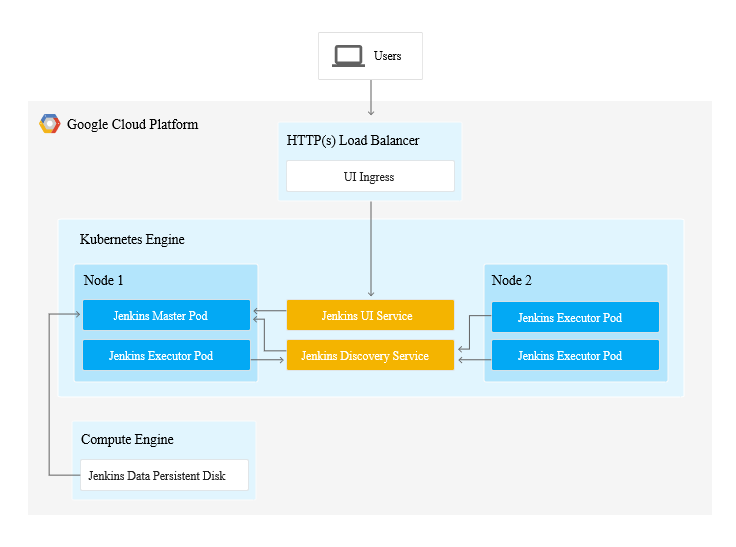
\includegraphics[width=1.0\textwidth]{gfx/jenkins-kubernetes-architecture.png}
 \caption{Deployment von Jenkins in einem Kubernetes Cluster mit mehreren Knoten \cite{Google:GKEJenkins}\label{fig:gkejenkins}}
\end{figure}

Google beschreibt in \cite{Google:GKEJenkins} einen Ansatz für eine skalierbare Architektur von Jenkins mit der \ac{GKE}.

In Abb. \ref{fig:gkejenkins} werden die Komponenten in mehreren Knoten, genannt Nodes zusammengefasst. In Node 1 befindet sich der Jenkins Master. Innerhalb dieses Nodes kann der Jenkins Master repliziert werden. Im gleichen Node oder in weiteren Nodes können die Jenkins Agenten, genannt Jenkins Executor, erzeugt werden.

Der Load Balancer aus der \ac{GKE} arbeitet vollautomatisch und erfordert nur wenige Parameter zur Konfiguration. Das reduziert den Aufwand in der Entwicklung dieser Architektur erheblich.

So lange in einem Node genug Ressourcen frei sind können weitere Container in so genannten Pods erzeugt werden. Zudem können beliebig viele weitere Nodes aktiviert oder erzeugt werden. Ein Node ist in \ac{GKE} eine virtuelle Maschine aus der Computing Engine.
\medskip
\\
Daraus resultiert eine hohe Flexibilität für die Skalierung der Anwendungen. Diese können sowohl vertikal anhand der Ressourcen von den Nodes, als auch Horizontal über die Aktivierung von weiteren Nodes oder Pods skaliert werden. Vor allem bestehen für die horizontale Skalierung mehrere Abstraktionsebenen.

\paragraph{Minikube}

\subsection{Anlegen eines Kubernetes Clusters für Jenkins}
Pathania beschreibt in \cite{Pathania2017}, wie Jenkins mit \ac{GCP} und Kubernetes und Docker skaliert werden kann. Hierbei geht er genau auf die Konfiguration von Kubernetes und der \ac{GCP} ein.



\paragraph{Jenkins Master-Agent Konfiguration}


\paragraph{Sonstige Konfigurationen}

\subsection{Jenkins Agents}

\paragraph{Virtuelle Maschinen}

\paragraph{Docker}

\paragraph{Minimale Images}

\subsection{Layering}

\section{Entwicklung von Docker-Images für Jenkins Agenten}

Während der Entwicklung eines Kubernetes Clusters für die \ac{SEU} gibt es viele Parameter, die sich ständig verändern können. Beispielsweise kann die Entscheidung für oder gegen eine Public-Cloud offen stehen oder es stehen Anpassungen offen. Daher kann nicht immer auf der größten Ebene angefangen werden.

Ein Ansatz für das Re-Design von Anwendungen ist die Entkernung und Modularisierung von Systemen \cite{Bussmann2006}.
Für einen gemeinsamen Nenner sollte die \ac{SEU} anhand ihrer wesentlichen Funktionen aufgeteilt werden \ref{jenkins:skalierung}. Dadurch kann anschließend die Entwicklung ihrer Komponenten parallel durchgeführt werden. 

\paragraph{Kleinster gemeinsamer Nenner der SEU}
Der kleinste gemeinsame Nenner der \ac{SEU} sind die einzelnen Stages aus den Pipelines, die nach dem Regelprozess für die Softwareentwicklung entwickelt wurden und die einzelnen Schritte aus dem Prozess darstellen.

Der größte Skalierungsbedarf besteht im Build-Stage, da sie sehr Rechen- und Speicherintensiv ist. Diese Komponente sollte als erstes optimiert werden.
Für die Build-Jobs gemäß der Pipeline ist die Plattform, in der sie sich befindet in erster Linie nicht relevant. 

\paragraph{Worauf es ankommt}
Die Build-Jobs werden in der Regel verteilt auf Agenten. Wichtig hierbei ist ihre Kommunikation zu den beteiligten Systemen. Beteiligte Systeme sind:
\begin{itemize}
    \item Versionsverwaltung: Sie verwaltet den Quellcode, der für den Build von ihr bezogen wird
    \item Artefaktrepository: Sie ist die Quelle, aus der Softwareartefakte bezogen werden und sichert und verfolgt die Ergebnisartefakte
    \item Integrationsplattform: Sie delegiert die Build-Jobs, welche die praktische Ausführung der Pipelines definieren
\end{itemize}

Agenten sind self-contained und werden in der Regel auf hierfür konfigurierten Maschinen ausgeführt. Daher kann bereits mit der Entwicklung von Images für die Agenten begonnen werden, während wichtige Aspekte des Gesamtsystems noch geklärt werden.

\paragraph{Vorteile von Container}
Container bieten klare Vorteile gegenüber klassischen VMs. 

\paragraph{Use-Case}
Die Images werden zur Erzeugung von Containern innerhalb eines Kubernetes Clusters für die Skalierung einer Komponente der Integrationsplattform Jenkins verwendet. Diese werden erzeugt, für den Einsatz als Agent innerhalb einer Master-Slave Konfiguration von Jenkins für verteilte Builds. Diese Agenten sind für die Ausführung eines Java Builds mit dem Build-Management Tool Maven zuständig.

\paragraph{Anforderungen}
\begin{itemize}
    \item Aufgrund von hohen Gebühren für cloud-out-traffic soll die Image möglichst klein sein
    \item Die Umgebung soll \ac{JDK11} und Maven enthalten und entsprechend konfiguriert werden
    \item Beim Bauen der Image sollen alle Ressourcen intern über eine private Artifactory-Instanz bezogen werden
    \item Zum Erstellen eines Builds soll Maven mit Artifactory kommunizieren und Daten übertragen können
    \item Zur Evaluation der Umgebung soll Maven einen erfolgreichen Build zu einem Testprojekt erstellen
\end{itemize}



\subsection{Auswahl eines Basis-Image}
Der erste Schritt in einem Dockerfile ist das Festlegen eines Basis-Images, aus welcher die Umgebung konfiguriert werden soll. Hierzu wird am Anfang der Dockerfile \lstinline{FROM image:tag} definiert. Theoretisch kann eine Image auch aus einer leeren Umgebung \lstinline{FROM scratch} erzeugt werden. Das ist jedoch unüblich, selbst bei Containern für embedded Systeme.

Hierzu gibt es im Docker-Hub öffentliche Images, die umkonfiguriert werden können. Die offizielle Maven image \lstinline{maven:3.6.3-jdk-11}, die Maven und JDK11 bereits installiert hat, könnte beispielsweise für eine einfache Anwendung verwendet werden. Für den Use-Case innerhalb der Continuous Integration Plattform können die potenziellen Basis-Images aus dem Dockerhub zwischen folgenden Stufen in ihrer Ausstattung unterschieden werden:
\begin{enumerate}
    \item Betriebssystem: \lstinline{ubuntu, debian, alpine}
    \item SDK: \lstinline{jdk11, openjdk11, adoptopenjdk11, amazoncoretto11}
    \item Build-Management: \lstinline{maven}
\end{enumerate}
Bei einer hohen Ausstattungsstufe besteht jedoch eine hohe Abhängigkeit von einer bestimmten Image, die wiederrum auf niedrigeren Stufen basiert. Für eine möglichst hohe Nachvollziehbarkeit wäre es sinnvoll eine möglichst niedrige Stufe zu wählen und die Umgebung innerhalb der eigenen Infrastruktur zu konfigurieren. Für eine möglichst hohe Effizienz der Container sind jedoch umfangreiche Kenntnisse über Betriebssysteme erforderlich. Diese fällt je nach Umfang in den Tätigkeitsbereich eines Systementwicklers.

\paragraph{Vorteile von selbst gebauten Images}
Für das Gesamtbild der Skalierbarkeit ist es jedoch sinnvoll das Ganze mit einer hohen Kompetenz anzugehen. Möglichst minimale und effiziente Container-Umgebungen wirken sich kumulativ auf den Ressourcenbedarf des ganzen Clusters aus. Bei einer Public-Cloud werden üblicherweise die genutzten Ressourcen mit einem Studensatz abgerechnet. Ein weiterer Vorteil entsteht durch das Prinzip des Layerings bei Container-Umgebungen. Auf einer eigenen Image können weitere Images basieren. Hierdurch muss lediglich eine Basis-Image entwickelt werden, in welchem nur die essentiellen Anpassungen vorgenommen werden, mit dem Ziel ein intern evaluiertes Betriebssystem bereitzustellen. Basierend hierauf können unabhängig voneinander Images aufbauen mit den entsprechenden Tools für die unterschiedlichen Programmiersprachen. Dadurch entsteht eine hohe Synergie und Flexibilität für die Systementwicklung und den Betrieb der Systeme.

\paragraph{Minimale Images}
Eine Best-Practice innerhalb der Entwicklung von Docker-Images ist ihre Größe so niedrig wie möglich zu halten. 

Die Linux-Image \lstinline{alpine} ist hierfür als Basis-Image besonders beliebt, da sie mit einer Größe von nur \lstinline{5 MB} eine Linux-Umgebung abbildet und eine Package-Repository besitzt \cite{docker-alpine}. Alpine benutzt jedoch nicht die C Standardlibrary \lstinline{glibc}, sondern \lstinline{musl libc} \cite{alpine-about}. Daher sollte die Nutzung gerade zum Kompilieren von Quellcode abgewägt werden.
Auch mit den offiziellen Docker-Images von Ubuntu und Debian kommt man auch mit entsprechenden Praktiken auf eine niedrige Größe. Für den Anwendungsfall innerhalb der \ac{CI} Plattform ist es wichtig eine kleinstmögliche Java Installation durchzuführen. Hierfür gibt es entsprechende \lstinline{slim} Editionen der JDK. 

Ein Vergleich zwischen der normalen \lstinline{openjdk:11-jdk} mit der \lstinline{-slim}\footnote{Vgl. Images aus index.docker.io}:
\begin{verbatim}
openjdk:11-jdk
SIZE 306.67 MB
sha256:9efbdac6886418e7c473ee4d59ff728d029fad773364cb671794333d-
d16e4158

openjdk:11-jdk-slim
SIZE 216.36 MB
sha256:a67455311b2982c4cb795c8a38d55cf17e840c8fdb9ca82d14cd38d8-
43e24111
\end{verbatim}

Beide Images basieren auf \lstinline{debian:buster}, wobei die zweite Image auf \lstinline{debian:buster-slim} basiert.

Ein vergleich zwischen \lstinline{alpine:3.12} und \lstinline{debian:buster-slim}
\begin{verbatim}
alpine:3.12
SIZE 2.3 MB
sha256:c929c5ca1d3f793bfdd2c6d6d9210e2530f1184c0f488f514f1bb808-
0bb1e82b

debian:buster-slim
SIZE 26.46 MB
sha256:9f8288b62780eaa2ee6341c6f8632990eae83d9b1caac9d0e4545e6f-
c8ce5e6d
\end{verbatim}

Auf die absolute Größe kommt es nicht an. Viel wichtiger ist es bei der Konfiguration der Images sich genau mit den Layers zu befassen. Jedes Befehl in der Dockerfile erzeugt einen neuen Layer. Das Löschen von Dateien wirkt sich nicht auf die vorigen Layer aus. Daher sollten Befehle verkettet als ein Befehl ausgeführt werden und möglichst wenige Daten erzeugt werden. 
\medskip
\\
Aufgrund der geringen Auswirkung der absoluten Größe wird möglichst auf eine Standardumgebung als Basis-Image verwendet. Hierfür wurde \lstinline{debian:buster-slim} ausgewählt. Die Debian Image auf Dockerhub ist eine offizielle Image, die hauptsächtlich vom Debian Maintainer tianon gepflegt und veröffentlicht wird \cite{docker-debian-builds, docker-debian}.

\paragraph{}{Konfiguration der Images}

\paragraph{Kommunikation mit Artifactory}

\paragraph{Bezug von Build-Tools über Artifactory}

\paragraph{Installation von Java}

\paragraph{Cacerts}

\paragraph{Installation von Maven}

\paragraph{Konfiguration von Maven}

\paragraph{Einfügen eines Testjobs}

\paragraph{Bauen von Images}

\paragraph{Evaluation der Images}

\paragraph{Bereitstellung der Images}

\paragraph{Integration in Jenkins}

\paragraph{SSH}

\paragraph{JNLP}